\input{preambuloSimple.tex}

%----------------------------------------------------------------------------------------
%	TÍTULO Y DATOS DEL ALUMNO
%----------------------------------------------------------------------------------------

\title{	
\normalfont \normalsize 
\textsc{\textbf{Estructura de Computadores (2016-2017)} \\ Subgrupo C3 \\ Grado en Ingeniería Informática\\ Universidad de Granada} \\ [25pt] % Your university, school and/or department name(s)
\horrule{0.5pt} \\[0.4cm] % Thin top horizontal rule
\huge Práctica 5: Caché \\ % The assignment title
\horrule{2pt} \\[0.5cm] % Thick bottom horizontal rule
}

\author{Mario Rodríguez Ruiz} % Nombre y apellidos

\date{\normalsize\today} % Incluye la fecha actual

%----------------------------------------------------------------------------------------
% DOCUMENTO
%----------------------------------------------------------------------------------------

\begin{document}

\maketitle % Muestra el Título

\newpage %inserta un salto de página

\tableofcontents % para generar el índice de contenidos

\listoffigures

\newpage

%----------------------------------------------------------------------------------------
%	Ejercicio 0
%----------------------------------------------------------------------------------------

\section{Procesador de las pruebas}

Se trata del procesador \textbf{Intel Pentium CPU 2020M de 2.40GHz}. 	

En la página de \textbf{Cpu-World} aparece muy bien detalladas sus características (\url{http://www.cpu-world.com/CPUs/Pentium_Dual-Core/Intel-Pentium%20Mobile%202020M.html}).
\\

La Figura \ref{fig:figura1} muestra la información básica de éste. 
	\begin{figure}[H] %con el [H] le obligamos a situar aquí la figura
		\centering
		\includegraphics[scale=0.7]{capturas/info1.png} 
		\caption{Primer indicio para averiguar la contraseña} 
		\label{fig:figura1}
	\end{figure}

Es ya en la Figura \ref{fig:figura2} donde aparece la información que interesa en este estudio. En ella puede los valores para los distintos niveles de caché, así como sus características.	
	
	\begin{figure}[H] %con el [H] le obligamos a situar aquí la figura
		\centering
		\includegraphics[scale=0.7]{capturas/info2.png} 
		\caption{Primer indicio para averiguar la contraseña} 
		\label{fig:figura2}
	\end{figure}
\vspace{-15pt}
\newpage

Otra forma de ver las características del cpu, pero esta vez desde la propia máquina, es mediante el comando \textbf{lscpu}.
La ejecución de éste en este estudio puede verse en la Figura \ref{fig:figura3}.
	\begin{figure}[H] %con el [H] le obligamos a situar aquí la figura
		\centering
		\includegraphics[scale=0.8]{capturas/lscpu.png} 
		\caption{Primer indicio para averiguar la contraseña} 
		\label{fig:figura3}
	\end{figure}

Una manera adicional de obtener las características de la caché desde la propia máquina es la que se ha proporcionado en el \textbf{Makefile} de esta misma práctica.
Su ejecución se muestra en la Figura \ref{fig:figura4}
	\begin{figure}[H] %con el [H] le obligamos a situar aquí la figura
		\centering
		\includegraphics[scale=1]{capturas/makeinfo.png} 
		\caption{Primer indicio para averiguar la contraseña} 
		\label{fig:figura4}
	\end{figure}
\newpage

\section{Tamaño de linea}

La parte del código \textbf{line.cc} que se ha modificado ha sido la siguiente:

\begin{lstlisting}
for(unsigned long long j = 0; j < line; j++)
	for (unsigned i = 0; i < bytes.size(); i += line)
		bytes[i]++;
\end{lstlisting}

Puede verse ésta en el código completo de a continuación:

\lstinputlisting{../v1/line.cc}

Después de la ejecución del programa \textbf{line} se ha obtenido, a través de \textbf{gnuplot}, la gráfica de la Figura \ref{fig:figura5}.
	\begin{figure}[H] %con el [H] le obligamos a situar aquí la figura
		\centering
		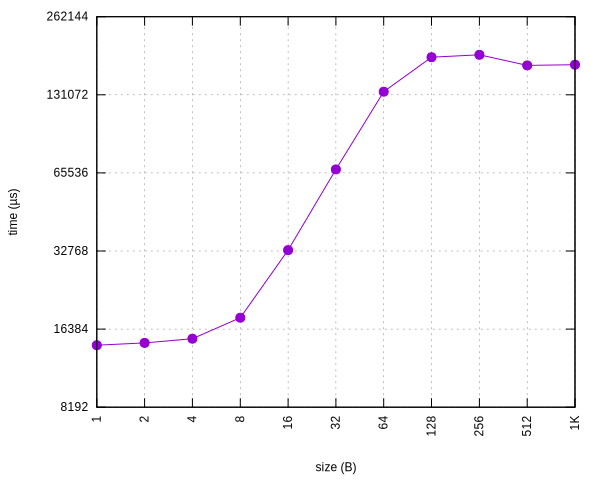
\includegraphics[scale=0.56]{capturas/line.png} 
		\caption{Resultado del tamaño de linea del procesador} 
		\label{fig:figura5}
	\end{figure}

En la gráfica puede verse el \textbf{incremento} de tiempo que hay desde \textbf{1B
hasta 64B}, esto se produce porque se obtienen muchos fallos de caché ya que se acceden a datos que no se encuentran en ella. Es por ello por lo que se tiene que tener en cuenta solo el bloque que los contiene de memoria principal. 
\\

Justo
después, los resultados se estabilizan cuando tenemos bastantes aciertos en caché. El pico donde se empieza a estabilizar es lo que se conoce como el \textbf{tamaño de línea de caché}, que en este caso es de \textbf{64B}.

\section{Tamaño de caché}

La parte del código \textbf{size.cc} que se ha modificado ha sido la siguiente:

\begin{lstlisting}
auto start = high_resolution_clock::now();

for (unsigned i = 0; i < STEPS; ++i)
	bytes[(i*64)&(size-1)]++;

auto stop = high_resolution_clock::now();

s = stop - start;
\end{lstlisting}

Puede verse ésta en el código completo de a continuación:

\lstinputlisting{../v1/size.cc}

Después de la ejecución del programa \textbf{size} se ha obtenido, a través de \textbf{gnuplot}, la gráfica de la Figura \ref{fig:figura6}.
\begin{figure}[H] %con el [H] le obligamos a situar aquí la figura
	\centering
	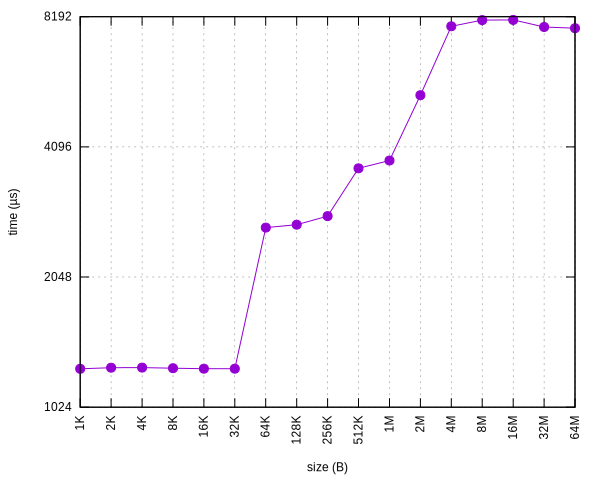
\includegraphics[scale=0.56]{capturas/size.png} 
	\caption{Resultado del tamaño de caché del procesador} 
	\label{fig:figura6}
\end{figure}

En la gráfica anterior puede observarse cómo se mantiene
\textbf{estable} el tiempo \textbf{desde 1K hasta 32K}. Justo después se tiene un incremento de tiempo significativo, producido porque se ha ocupado todo el espacio de la \textbf{caché
L1} y ya se está accediendo a la \textbf{L2}. Ese incremento en el tiempo (produciendo un pico) indica que el \textbf{tamaño de la caché L1 es de 32KB}.\\

El tiempo desde \textbf{64K hasta 256K es estable}, pero justo a continuación
se obtiene un incremento de tiempo importante que indica que la L2 se ha
ocupado por completo y se empezará a usar la L3. El pico de subida creado por 
este incremento muestra que el \textbf{tamaño de la caché L2 es de 256K}.\\

Posteriormente, \textbf{desde 512k hasta poco antes de 2M} se obtienen resultados estables de nuevo. La conclusión de esta estabilidad indica que la cache L3 se ha ocupado por completo y, a partir de este momento,
los accesos se realizarán sobre memoria principal. Es por ello por lo que se puede afirmar que la caché \textbf{L3
es de 2M}.
\\

La presentación de estos datos puede ayudar a entender la importancia que tienen tamaños de caches que, cuanto más lejos del procesador más tiempo
existe de acceso a datos. Es por ello por lo que la L1 es la más rápida y la memoria
principal la más lenta.


\newpage

\end{document}
